\documentclass[11pt]{article}

% "preprint" = wersja z nazwiskami i numerami stron (do oddawania etapów kursu).
\usepackage[preprint]{acl}

\usepackage{times}
\usepackage{latexsym}
\usepackage[T1]{fontenc}
\usepackage[utf8]{inputenc}
\usepackage{microtype}
% inconsolata (font \texttt) jest w texlive-fonts-extra (1,8 GB); bez niego lokalnie wychodzi domyślny font.
\IfFileExists{inconsolata.sty}{\usepackage{inconsolata}}{}
\usepackage{xcolor}
\usepackage{graphicx}
\usepackage{booktabs}
\usepackage{amsmath}
\usepackage{tabularx}
\newcolumntype{L}[1]{>{\raggedright\arraybackslash}p{#1}}
\newcolumntype{Y}{>{\raggedright\arraybackslash}X}

% Widoczny znacznik luki. Przed oddaniem: \renewcommand{\todo}[1]{} ukrywa wszystkie.
\newcommand{\todo}[1]{{\color{red}[TODO: #1]}}

\graphicspath{{rysunki/}}

\title{Who Lives in This Building? An Agentic VLM System for Building-Level Population Estimation in Wrocław}

% Pięć osób z jedną afiliacją: imiona w dwóch rzędach, afiliacja i kontakt pod spodem.
\author{
  \textbf{Stanisław Brzezicki},
  \textbf{Dominik Czech},
  \textbf{Michał Jankowski},
\\
  \textbf{Kacper Janus},
  \textbf{Mateusz Wechman}
\\
\\
  Wrocław University of Science and Technology
\\
  \small{
    \textbf{Correspondence:} \texttt{email@domain}
  }
}

\begin{document}
\maketitle

\begin{abstract}
Traffic models need the people who actually live in each building, but the Polish census reports only registered residents per 125\,m cell.
In our system a vision-language model (VLM) looks at a building in oblique aerial photos and reads its record from the national building database; a formula with constants from the literature computes residents, and the VLM reweights it with two multipliers, the residential share and the density.
A second model questions the VLM where totals disagree with the census, which it treats as a lower bound, and a third searches the web for the number of beds or flats in the largest buildings.
On a test area of three sheets (680 buildings) with a cheap model, Claude Haiku, the regional totals reach 103\% of SRLM in the three regions the area fully covers, against 55\% for a volume baseline that inherits the census total; per region the ratio ranges from 0.96 to 1.26.
The final run covers the whole city with an open-weight VLM and is evaluated once against an independent estimate of actual residents.
\end{abstract}

\section{Introduction}

We estimate how many people actually live in each building in Wrocław, as input to a traffic model.
The 2021 census (NSP) counts people at their registered address and stops at 125\,m cells, so it misses many students and migrants; an estimate of actual residents, SRLM \citep{szmytkie2023srlm}, is 33\% higher but given only for 375 regions.
A VLM, the witness, reports what it sees and a fixed formula computes the residents, so every estimate can be traced to a description and a constant; a second model, the balancing agent, can ask the witness to look again.

We ask how close the regional totals come to SRLM and where they diverge (RQ1), whether the census loop changes the descriptions for the better (RQ2), and whether an open-weight VLM can replace a paid one (RQ3).
So far we ran the pipeline on a cheap paid model, Claude Haiku; the final run uses the open-weight Qwen3.8-27B \citep{qwen2026}.

\section{Related Work}

Dasymetric mapping redistributes counts using footprint or volume \citep{mennis2003generating,lwin2009gis,ural2011building}, also on BDOT10k, the Polish building database \citep{calka2016redistribution}.
In Kraków, a fit on BDOT10k gross floor area (footprint $\times$ storeys) to registered residents gives 2.88 residents per single-family house and 37\,m$^2$ per resident in multi-family buildings \citep{pirowski2018detailed}; the floor area includes shops and staircases, and the authors name the varying share of non-residential space as the open problem.
On a 1\,km grid the best map uses the same values \citep{pirowski2024dasymetric}, as far as its abstract shows (no full-text access).
On street-level images, zero-shot GPT-4o errs by 2.4 storeys \citep{openfacades2025}, and images add most for type and function but not for population, with predictions following a conflicting record \citep{tan2026streetview}.
Floor counts have been estimated from geodata alone \citep{moubayed2025floors}; three non-systematic searches found no evaluation of VLMs on oblique aerial imagery.
Debating agents can converge on wrong answers \citep{du2024debate}, and unchecked independent agents amplified errors 17.2 times against 4.4 with centralized verification \citep{kim2025scaling}, so our loop flags discrepancies without enforcing agreement.

\section{Data}

We use public sources: an oblique orthophoto from 2025 (each sheet photographed at an angle from N, E, S and W, 5\,cm pixel), BDOT10k (footprint, function, storeys, state), airborne laser scanning (height), OpenStreetMap address points (imported from the national register) and the census (residents per cell).
The test area is three sheets around Grunwaldzki Square, 1.2\,km$^2$ with 680 buildings, 434 of them residential, mostly tenements and blocks, with few houses; we chose the sheets so that they fully cover three SRLM regions (Figure~\ref{fig:dane}).

The photos are georeferenced, so a building gets up to 4 views and 4 facades, which are crops with a wall rectified to a rectangle (Figure~\ref{fig:karta}); buildings at the outer edge get fewer views or only the record.
Height is the median of the national laser-scanning surface model inside the footprint minus the terrain model.
The roof lies 0.96\,$\times$\,height from the base: we matched roof texture across the four views and divided the shift by that height (median over 61 buildings).

SRLM \citep{szmytkie2023srlm} estimates actual residents at the end of 2022, 893,506 in the city, from registrations, dwelling counts and dormitory beds, and uses BDOT10k floor area only in a few regions without registrations.
No agent sees it.

\begin{figure*}[t]
  \centering
  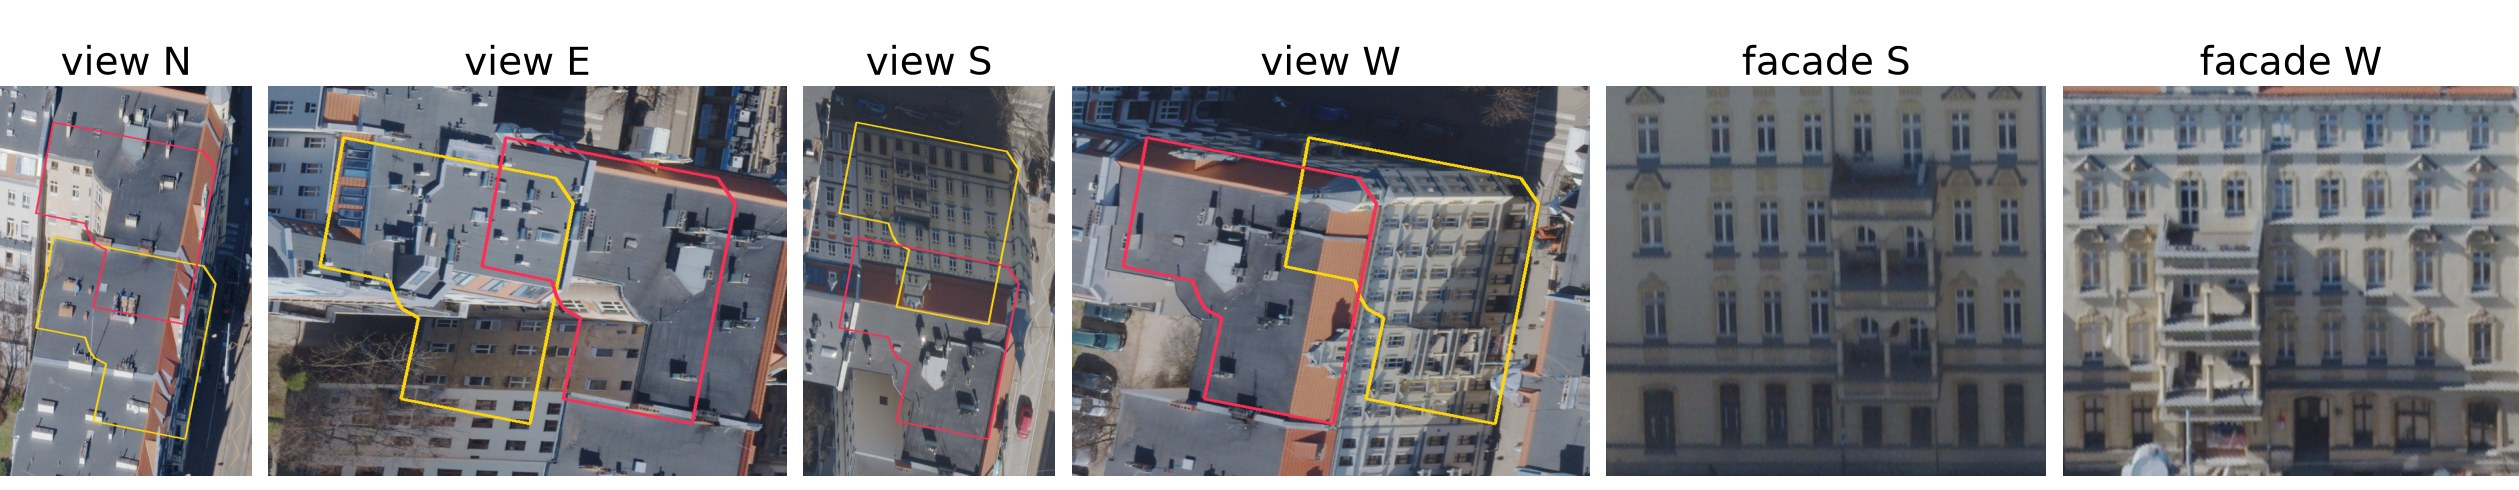
\includegraphics[width=\textwidth]{karta}
  \caption{What the witness gets for a tenement at Piastowska 36: views with base (yellow) and roof (red) outlines, and rectified facades.}
  \label{fig:karta}
\end{figure*}

\begin{figure*}[t]
  \centering
  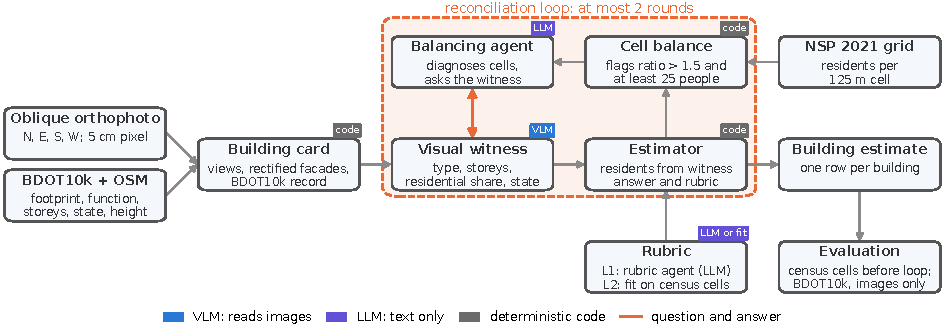
\includegraphics[width=\textwidth]{architektura}
  \caption{The system. The witness, the balancing agent and the search agent call a model; the rest is deterministic code.}
  \label{fig:architektura}
\end{figure*}

\begin{figure}[t]
  \centering
  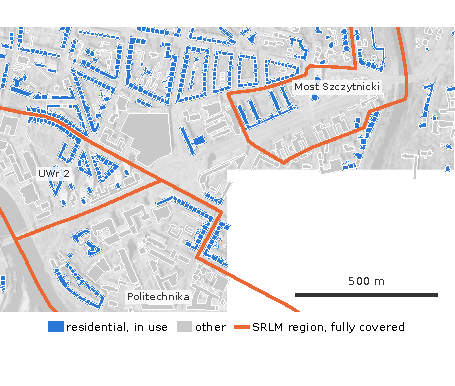
\includegraphics[width=\columnwidth]{dane}
  \caption{The three test sheets: residential buildings from BDOT10k and the SRLM regions they fully cover.}
  \label{fig:dane}
\end{figure}

\section{System}

Figure~\ref{fig:architektura} shows the system.
Each agent is one stateless model call answering in JSON forced by a schema, and code holds the state.
The code calls Claude through its API or any VLM served by vLLM, logs every call, retries a call without valid JSON up to five times, and resumes an interrupted run; the prompts, in Polish, are in the repository.

\paragraph{Witness.}
It gets the images, the BDOT10k record and the residents the formula gives for the record's class, and returns, in this order, a rationale, whether signs of dwellings are visible (laundry or plants on balconies, varied curtains, satellite dishes), the type, the state, the residential share and the density, but not residents.
Both multipliers are 1 for a typical building of the class, ordinary ground-floor shops included; the share drops only when whole upper floors look non-residential, and the density moves only for visible reasons, which the prompt lists for Polish cities (micro-apartments and workers' hostels up, large tenement flats and boarded-up windows down).
A building that BDOT10k lists as non-residential gets residents only with visible signs of dwellings and a confidence of at least 0.6, because on ambiguous images the witness tended to answer ``tenement, share 0.5''.

\paragraph{Formula.}
A building not in use, or of a type without flats, gets 0.
Otherwise:
\begin{align*}
  \text{house} &= \text{residents per house} \times \text{share} \times \text{density} \\
  \text{other} &= \frac{\text{footprint} \times \text{storeys} \times \text{share} \times \text{density}}{\text{m}^2\text{ per person}}
\end{align*}
Footprint and storeys come from BDOT10k, which has storeys for every residential building.
Table~\ref{tab:rubryka} gives the constants.
The first two come from Kraków, with the same database and similar housing (GUS, 2024: 33.4\,m$^2$ of usable area per person there, 34.6\,m$^2$ in Wrocław); the third, from a US trade survey, is the weakest.

\begin{table}[t]
  \centering
  \footnotesize
  \begin{tabularx}{\columnwidth}{@{}llY@{}}
    \toprule
    Class & Value & Source \\
    \midrule
    House & 2.88 residents & \citet{pirowski2018detailed}, Table 1 \\
    Multi-family & 37.08\,m$^2$ per person & same \\
    Collective & 31\,m$^2$ per bed & \citet{abramson2014home} \\
    \bottomrule
  \end{tabularx}
  \caption{The rubric: three constants in the code.}
  \label{tab:rubryka}
\end{table}

\paragraph{Loop.}
In at most two rounds, code flags a census cell whose estimate differs from the census more than 1.5 times and by at least 25 people, counting only cells with an estimate for every residential building.
The agent, told that the census counts registered residents and is almost certainly too low, reads the flagged cells and the buildings where the witness contradicts the record, and chooses what to ask; it sees no images, changes no numbers, and a filter strips digits from its questions.
The witness changes its answer only if the image justifies it, and the formula recomputes every estimate.

\paragraph{Search agent.}
Most residents sit in a few large buildings.
For every dormitory, boarding school and hotel in BDOT10k and for 4 more of the largest buildings per sheet, a model with web search looks for a published number of beds or flats for that very building, in at most 2 searches.
Hotels are included because private dormitories with micro-apartments are registered as hotels; a studio counts as one bed and a tourist hotel as none.
Touching segments with the same function are searched together and the number is split by floor area; segments without an address of their own are skipped, because with a neighbour's address they found its beds again.
Beds replace the estimate and flats count 1.71 persons (GUS, Wrocław 2024).

\paragraph{One building.}
A dormitory at Piastowska 1 (1,466.6\,m$^2$, 8 storeys) is collective housing with both multipliers 1, so 1,466.6 $\times$ 8 / 31 = 378 residents; its cell has 33 people in the census and is flagged, but the agent blames the constant and asks nothing.
The search agent finds 802 beds for both segments of the dormitory, and this one gets 674 by floor area.

\section{Evaluation}

We have no true count for a single building, so we compare regional sums with SRLM, once, after the run on the whole city.
A region counts if its residential floor area (BDOT10k, footprint $\times$ storeys) has an estimate for at least 95\%, and a building on a border counts by the share of its footprint.
The \textbf{level} is the estimated total divided by the SRLM total.
\textbf{Spearman} compares only the order of regions (1: same order, 0: no relation).
\textbf{WAPE} rescales the estimates to the SRLM total and divides the sum of absolute errors by that total: reference 100, 100 with estimates 150, 50 gives 0.5, and half of WAPE is the share of people in the wrong region.
We also list the regions with the largest and smallest ratio to SRLM and read them for causes, such as estates built after 2022, which our 2025 photos show and SRLM does not.
References without a model: the census split between regions by area, and building volume $\times$ BDOT (0 for buildings not residential or not in use), which distributes the census population by volume.

\section{Results on Three Sheets}

Haiku 5.5 processed 680 buildings for 1.06 USD, with no fallback to the record, and estimates 21,139 residents (Figure~\ref{fig:szacunki}).
The share is 1 for 425 of 434 residential buildings and the density 1 for 413, above 1 for 7 and below 1 for 14; non-residential buildings in BDOT10k got residents in 6 cases, against 25 (789 residents) with the earlier prompt without the check for signs of dwellings.
The loop flagged 25 of 46 cells, almost all above the census (17,388 against 10,629 residents), asked about 10 buildings and changed 4 answers, among them a university building first described as a dormitory with 237 residents.
The search agent found numbers for 6 of 17 buildings, including the hotel at wybrzeże Pasteura 18, which turned out to be the Starter micro-apartments with 170 units (counted as flats, which overstates studios); for a complex of three dormitories it found only two and gave no number.

\begin{table}[t]
  \centering
  \footnotesize
  \begin{tabular}{@{}lll@{}}
    \toprule
    Estimate & Level & WAPE \\
    \midrule
    Census split by area & 0.45 & 0.43 \\
    Volume $\times$ BDOT & 0.55 & 0.21 \\
    System, before loop & 1.04 & 0.15 \\
    System, final & 1.03 & 0.10 \\
    \bottomrule
  \end{tabular}
  \caption{Sums against SRLM in the three fully covered regions (7,869 residents).}
  \label{tab:wyniki}
\end{table}

Against SRLM the level is close to 1, while the baseline and the census stay far below (Table~\ref{tab:wyniki}).
Per region the ratio is 0.96 (UWr 2), 1.26 (Politechnika) and 0.97 (Most Szczytnicki).
In Politechnika the estimate equals the rubric applied to the BDOT10k record: tenements at 37.08\,m$^2$ per person already exceed SRLM for the whole region, and monasteries at 31\,m$^2$ per person add about 300.
With three regions this shows only that the evaluation works and where to look; we do not tune prompts on them.

\begin{figure}[t]
  \centering
  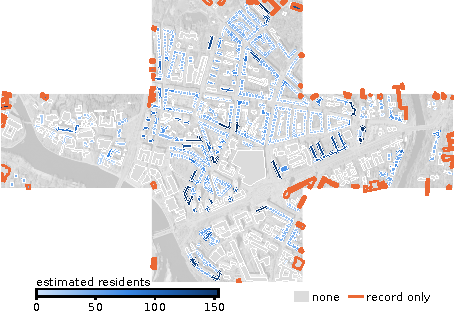
\includegraphics[width=\columnwidth]{szacunki}
  \caption{Estimated residents per building on the three sheets. An estimate, not a measurement.}
  \label{fig:szacunki}
\end{figure}

\section{Plan}

The final run covers the whole city: 826 sheets from the 2025 flight, which cover 99.97\% of Wrocław, with 70,322 buildings in BDOT10k.
The witness and the balancing agent run on Qwen3.8-27B on our own server; the search agent stays on Claude Haiku, which has web search.
First Qwen runs on the three test sheets and we compare its descriptions and totals with Haiku on the same buildings (RQ3); then prompts and constants are frozen, and SRLM is evaluated once on all regions that pass the coverage rule, before and after the loop (RQ1, RQ2).
Thresholds and limits of the loop and the search agent are starting values, to be set with domain experts.

\section{Limitations}

A per-building number is the output of a formula, not a measurement.
The evidence so far is one district with three regions, each run was done once, although identical runs at temperature 0 can differ in accuracy by up to 15\% \citep{atil2024nondeterminism}.
The constants come from another city, were fitted to registered rather than actual residents and, for collective housing, come from another country.
SRLM is itself an estimate for 2022, the census is from 2021 and the photos from 2025, and SRLM takes dormitory beds from the web, as our search agent may.

Code and notebooks: \url{https://github.com/wust-terrain/wroclaw-population-agents}.
\todo{authors: add an AI-use statement and verify all sources. Drafted with Claude Code and Scientific Agent Skills (Kassis et al., 2026, arXiv:2609.00065).}

% Bibliografia wklejona, żeby nie dodawać pliku .bib. Metadane sprawdzone w Crossref, OpenAlex, na arXiv i Hugging Face.
\begin{thebibliography}{15}
\providecommand{\natexlab}[1]{#1}

\bibitem[{Abramson(2014)}]{abramson2014home}
Paul Abramson. 2014.
\newblock A home away from home: 2014 college housing report.
\newblock \emph{College Planning \& Management}, May:20--27.

\bibitem[{Atil et~al.(2024)}]{atil2024nondeterminism}
Berk Atil, Sarp Aykent, Alexa Chittams, Lisheng Fu, and others. 2024.
\newblock Non-determinism of ``deterministic'' {LLM} settings.
\newblock ArXiv:2408.04667.

\bibitem[{Ca{\l}ka et~al.(2016)Ca{\l}ka, Bielecka, and
  Zdunkiewicz}]{calka2016redistribution}
Beata Ca{\l}ka, El{\.z}bieta Bielecka, and Katarzyna Zdunkiewicz. 2016.
\newblock \href {https://doi.org/10.1515/geocart-2016-0011} {Redistribution
  population data across a regular spatial grid according to buildings
  characteristics}.
\newblock \emph{Geodesy and Cartography}, 65(2):149--162.

\bibitem[{Du et~al.(2024)Du, Li, Torralba, Tenenbaum, and
  Mordatch}]{du2024debate}
Yilun Du, Shuang Li, Antonio Torralba, Joshua~B. Tenenbaum, and Igor Mordatch.
  2024.
\newblock Improving factuality and reasoning in language models through
  multiagent debate.
\newblock In \emph{Proceedings of the 41st International Conference on Machine
  Learning (ICML)}, volume 235 of \emph{PMLR}.
\newblock ArXiv:2305.14325.

\bibitem[{Kim et~al.(2025)}]{kim2025scaling}
Yubin Kim, Ken Gu, and others. 2025.
\newblock Towards a science of scaling agent systems.
\newblock ArXiv:2512.08296.

\bibitem[{Liang et~al.(2025)Liang, Xie, Zhao, Stouffs, and
  Biljecki}]{openfacades2025}
Xiucheng Liang, Jinheng Xie, Tianhong Zhao, Rudi Stouffs, and Filip Biljecki.
  2025.
\newblock {OpenFACADES}: An open framework for architectural caption and
  attribute data enrichment via street view imagery.
\newblock \emph{ISPRS Journal of Photogrammetry and Remote Sensing},
  230:918--942.
\newblock ArXiv:2504.02866.

\bibitem[{Lwin and Murayama(2009)}]{lwin2009gis}
Ko~Ko Lwin and Yuji Murayama. 2009.
\newblock \href {https://doi.org/10.1111/j.1467-9671.2009.01171.x} {A {GIS}
  approach to estimation of building population for micro-spatial analysis}.
\newblock \emph{Transactions in GIS}, 13(4):401--414.

\bibitem[{Mennis(2003)}]{mennis2003generating}
Jeremy Mennis. 2003.
\newblock \href {https://doi.org/10.1111/0033-0124.10042} {Generating surface
  models of population using dasymetric mapping}.
\newblock \emph{The Professional Geographer}, 55(1):31--42.

\bibitem[{Moubayed et~al.(2025)Moubayed, Becker, and
  Blankenbach}]{moubayed2025floors}
Fadi Moubayed, Ralf Becker, and J{\"o}rg Blankenbach. 2025.
\newblock \href {https://doi.org/10.1080/10095020.2025.2465307} {Geodata-based
  number of floor estimation for urban residential buildings as an input
  parameter for energy modelling}.
\newblock \emph{Geo-spatial Information Science}, 28(5):2525--2551.

\bibitem[{Pirowski and Bartos(2018)}]{pirowski2018detailed}
Tomasz Pirowski and Karolina Bartos. 2018.
\newblock \href {https://doi.org/10.15292/geodetski-vestnik.2018.03.458-471}
  {Detailed mapping of the distribution of a city population based on
  information from the national database on buildings}.
\newblock \emph{Geodetski vestnik}, 62(3):458--471.

\bibitem[{Pirowski and Szypu{\l}a(2024)}]{pirowski2024dasymetric}
Tomasz Pirowski and Bart{\l}omiej Szypu{\l}a. 2024.
\newblock \href {https://doi.org/10.1080/24694452.2024.2313500} {Dasymetric
  population mapping using building data}.
\newblock \emph{Annals of the American Association of Geographers},
  114(5):1001--1019.

\bibitem[{Qwen Team(2026)}]{qwen2026}
Qwen Team. 2026.
\newblock {Qwen3.8-27B}.
\newblock Model card, \url{https://huggingface.co/Qwen/Qwen3.8-27B}.

\bibitem[{Szmytkie et~al.(2023)}]{szmytkie2023srlm}
Robert Szmytkie, Piotr Kryczka, Agnieszka Lisowska-Kierepka, and Katarzyna Kuzara. 2023.
\newblock Szacowanie rzeczywistej liczby mieszkańców Wrocławia.
\newblock Report for the City of Wrocław, University of Wrocław, \url{https://bip.um.wroc.pl/artykul/565/70661}.

\bibitem[{Tan(2026)}]{tan2026streetview}
Kaizhen Tan. 2026.
\newblock Seeing the city or recognizing the place? {What} street-view imagery
  adds beyond existing urban data in {VLM}-based urban sensing.
\newblock ArXiv:2610.00031.

\bibitem[{Ural et~al.(2011)Ural, Hussain, and Shan}]{ural2011building}
Serkan Ural, Ejaz Hussain, and Jie Shan. 2011.
\newblock \href {https://doi.org/10.1016/j.jag.2011.06.004} {Building
  population mapping with aerial imagery and {GIS} data}.
\newblock \emph{International Journal of Applied Earth Observation and
  Geoinformation}, 13(6):841--852.

\end{thebibliography}

\end{document}
